
%%%%%%%%%%%%%%%%%%%%%%%%%%%%%%%%%%%%%%%%%%%%%%%%%%%%%%%%%%%%%%%%%%%%%
%% This is a (brief) model paper using the achemso class
%% The document class accepts keyval options, which should include
%% the target journal and optionally the manuscript type.
%%%%%%%%%%%%%%%%%%%%%%%%%%%%%%%%%%%%%%%%%%%%%%%%%%%%%%%%%%%%%%%%%%%%%
\documentclass[journal=jacsat,manuscript=article]{achemso}

%%%%%%%%%%%%%%%%%%%%%%%%%%%%%%%%%%%%%%%%%%%%%%%%%%%%%%%%%%%%%%%%%%%%%
%% Place any additional packages needed here.  Only include packages
%% which are essential, to avoid problems later. Do NOT use any
%% packages which require e-TeX (for example etoolbox): the e-TeX
%% extensions are not currently available on the ACS conversion
%% servers.
%%%%%%%%%%%%%%%%%%%%%%%%%%%%%%%%%%%%%%%%%%%%%%%%%%%%%%%%%%%%%%%%%%%%%
\usepackage[version=3]{mhchem} % Formula subscripts using \ce{}
\usepackage[T1]{fontenc}       % Use modern font encodings

%%%%%%%%%%%%%%%%%%%%%%%%%%%%%%%%%%%%%%%%%%%%%%%%%%%%%%%%%%%%%%%%%%%%%
%% If issues arise when submitting your manuscript, you may want to
%% un-comment the next line.  This provides information on the
%% version of every file you have used.
%%%%%%%%%%%%%%%%%%%%%%%%%%%%%%%%%%%%%%%%%%%%%%%%%%%%%%%%%%%%%%%%%%%%%
%%\listfiles

%%%%%%%%%%%%%%%%%%%%%%%%%%%%%%%%%%%%%%%%%%%%%%%%%%%%%%%%%%%%%%%%%%%%%
%% Place any additional macros here.  Please use \newcommand* where
%% possible, and avoid layout-changing macros (which are not used
%% when typesetting).
%%%%%%%%%%%%%%%%%%%%%%%%%%%%%%%%%%%%%%%%%%%%%%%%%%%%%%%%%%%%%%%%%%%%%
\newcommand*\mycommand[1]{\texttt{\emph{#1}}}
\usepackage{color}
\def\todo#1{{\color{red}[TODO: #1]}}




%%%%%%%%%%%%%%%%%%%%%%%%%%%%%%%%%%%%%%%%%%%%%%%%%%%%%%%%%%%%%%%%%%%%%
%% Meta-data block
%% ---------------
%% Each author should be given as a separate \author command.
%%
%% Corresponding authors should have an e-mail given after the author
%% name as an \email command. Phone and fax numbers can be given
%% using \phone and \fax, respectively; this information is optional.
%%
%% The affiliation of authors is given after the authors; each
%% \affiliation command applies to all preceding authors not already
%% assigned an affiliation.
%%
%% The affiliation takes an option argument for the short name.  This
%% will typically be something like "University of Somewhere".
%%
%% The \altaffiliation macro should be used for new address, etc.
%% On the other hand, \alsoaffiliation is used on a per author basis
%% when authors are associated with multiple institutions.
%%%%%%%%%%%%%%%%%%%%%%%%%%%%%%%%%%%%%%%%%%%%%%%%%%%%%%%%%%%%%%%%%%%%%

\author{Robert O. Ness}
\email{nessr@purdue.edu}
\affiliation[Purdue University]{Purdue University Department of Statistics, West Lafayette}
\alsoaffiliation[Northeastern University]{College of Science, College of Computer and Information Science, Northeastern University, Boston}
\affiliation[Northeastern University]{College of Science, College of Computer and Information Science, Northeastern University, Boston}
\author{Karen Sachs}
\affiliation[Stanford University]{School of Medicine, Stanford University, Palo Alto}
\author{Olga Vitek}
\affiliation[Northeastern University]{College of Science, College of Computer and Information Science, Northeastern University, Boston}



%%%%%%%%%%%%%%%%%%%%%%%%%%%%%%%%%%%%%%%%%%%%%%%%%%%%%%%%%%%%%%%%%%%%%
%% The document title should be given as usual. Some journals require
%% a running title from the author: this should be supplied as an
%% optional argument to \title.
%%%%%%%%%%%%%%%%%%%%%%%%%%%%%%%%%%%%%%%%%%%%%%%%%%%%%%%%%%%%%%%%%%%%%
 \title[]
   {From correlation to causality: statistical approaches to learning regulatory relationships in large-scale biomolecular investigations}

%%%%%%%%%%%%%%%%%%%%%%%%%%%%%%%%%%%%%%%%%%%%%%%%%%%%%%%%%%%%%%%%%%%%%
%% Some journals require a list of abbreviations or keywords to be
%% supplied. These should be set up here, and will be printed after
%% the title and author information, if needed.
%%%%%%%%%%%%%%%%%%%%%%%%%%%%%%%%%%%%%%%%%%%%%%%%%%%%%%%%%%%%%%%%%%%%%
\abbreviations{IR,NMR,UV}
\keywords{causal inference, big data, causal networks, Bayesian networks}

%%%%%%%%%%%%%%%%%%%%%%%%%%%%%%%%%%%%%%%%%%%%%%%%%%%%%%%%%%%%%%%%%%%%%
%% The manuscript does not need to include \maketitle, which is
%% executed automatically.
%%%%%%%%%%%%%%%%%%%%%%%%%%%%%%%%%%%%%%%%%%%%%%%%%%%%%%%%%%%%%%%%%%%%%
\begin{document}

\begin{abstract}
  Causal inference -- the task of uncovering regulatory relationships between components of biomolecular pathways and networks - is a primary goal of many high throughput investigations.  Statistical associations between quantitative measurements can reveal an enticing number of putative causal interactions, but when do such associations reflect the underlying causal biomolecular mechanisms?  The goal of this perspective is to provide suggestions for causal inference in large scale experiments, which utilize high throughput technologies such as mass spectrometry-based proteomics.  We describe in non-technical terms the pitfalls of inference in large datasets, and suggest methods to overcome these pitfalls and reliably find regulatory associations.
\end{abstract}

%%%%%%%%%%%%%%%%%%%%%%%%%%%%%%%%%%%%%%%%%%%%%%%%%%%%%%%%%%%%%%%%%%%%%
%% Start the main part of the manuscript here.
%%%%%%%%%%%%%%%%%%%%%%%%%%%%%%%%%%%%%%%%%%%%%%%%%%%%%%%%%%%%%%%%%%%%%
\section{Introduction}

Causal inference \cite{pearl2009causality} applied to 'omics experiments, elucidates statistical associations (e.g. Pearson correlation, Spearman correlation, mutual information), which result from the underlying biomolecular mechanistic relationships. Modern high-throughput technologies such as mass spectrometry-based proteomics quantify components of the biomolecular systems on a large scale. We will demonstrate the paradoxical result that the large amount of data generated by these experiments make the task of causal inference more difficult.  If only two biologically unrelated analytes were measured simultaneously, there is some probability of a spurious association -- an association between the analytes arising purely from random chance -- though the chance of this happening is low and gets lower as sample size increases. The difficulty of high-throughput data stems from the fact that the more analytes that are measured, the more pairwise associations between analytes are generated, resulting in a much greater chance for the appearance of spurious associations that are just as strong as associations that represent actual biological relationships.  This obfuscates the true signal, leading to increased false discoveries of putative causal events.  This problem can be addressed by refining the biological question, and by improving experimental design in terms of selection of  (1) the subset of analytes, (2) the number of biological replicates, and (3) the type of biological conditions and stresses. Below, we describe in non-technical terms the process of elucidating causal associations from high-throughput data and suggest practical approaches for analysis of large scale datasets. 


\section{I. Small-scale statistical inference of causal relationships: conditional independence and interventions}

\begin{figure}[!tpb]
\centerline{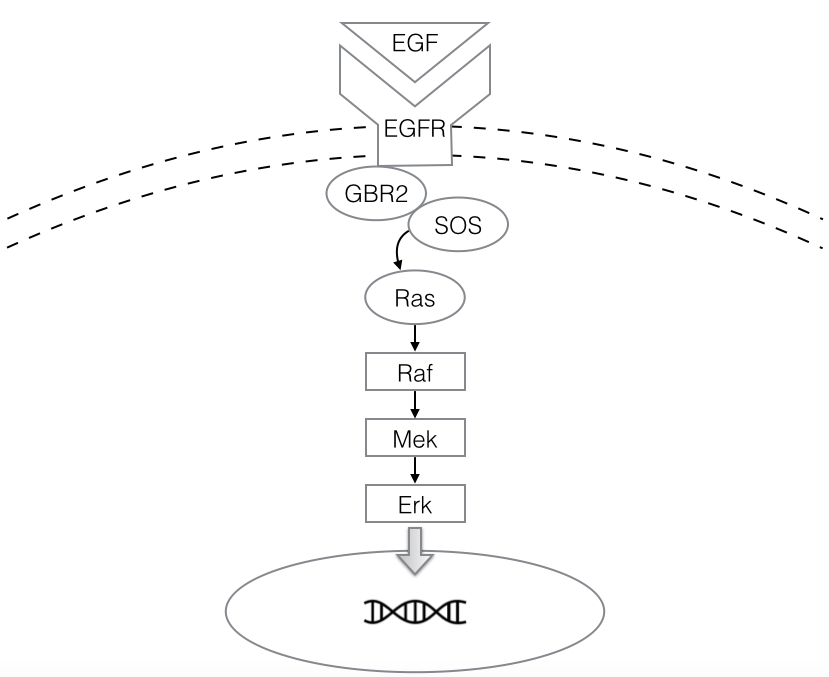
\includegraphics[width=.5\textwidth]{figs/egfr.png}}
\caption{EGFR MAPK signaling pathway, an example of a pathway containing the phosphorylation cascade from Raf to Mek to Erk.  The binding of ligand EGF to EGFR initiates a signal that leads to the cascade, which in turn regulates transcription.  This cascade implies two direct causal relationships, namely Raf --> MEK, and Mek --> Erk.  Raf and Erk have an indirect causal relationship, through Mek.\label{mapk}}
\end{figure}

Consider, e.g. the MAPK signaling cascade in Figure \ref{mapk}, which is part of several signaling pathways such as the EGFR MAPK pathway\cite{holbro2004erbb}. In this cascade Raf causally affects the level of active (i.e., phosphorylated) Mek, while Mek causally affects Erk. Imagine these causal relationships were unknown: could they be detected from quantitative measurements on these phosphoproteins?  

To illustrate the process of causal inference in this context, we simulated artificial data using the computational Huang-Ferrell model \cite{huang1996ultrasensitivity} of this cascade. The model represents the key binding, phosphorylation, and dephosphorylation reactions of the cascade with mass action kinetics, and replicates the MAPK key signaling behavior observed in nature.  We used the model to simulate an experiment with 50 replicate biological samples, and measurements of concentration (umol) of phosphorylated Raf, and doubly phosphorylated Mek and Erk in each sample. 

\begin{figure}[!tpb]
\centerline{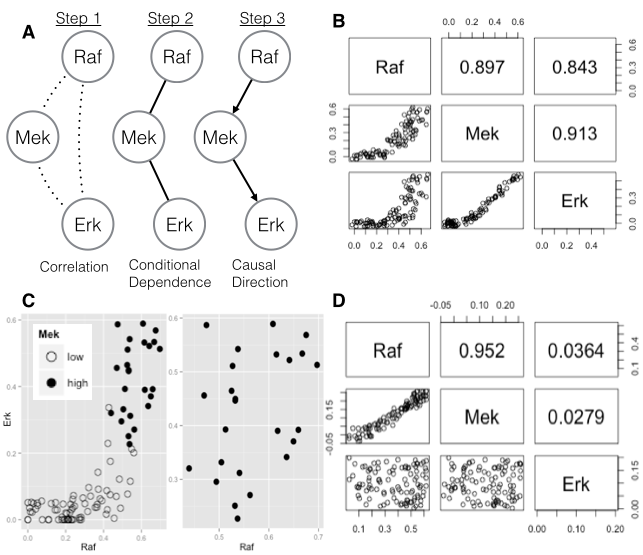
\includegraphics[width=1\textwidth]{figs/mapk.png}}
\caption{A: Overview of the 3 steps of causal inference, illustrated for the MAPK signaling cascade.    B, C, and D feature an experiment simulated from the Huang-Ferrell computational model of the phosphorylation cascade.  B: Pairwise plots of concentration values of phosphorylated (doubly phosphorylated for Mek and Erk) forms of each protein, and observed Spearman correlation values.  The Raf -- Erk correlation is high, despite the fact that Raf does not directly regulate Erk.  C: Concentrations of Raf versus Erk, where samples corresponding to high Mek are highlighted in circles.  The right panel of B shows the subset of samples with high Mek (i.e. conditional on Mek being high). In these samples the association between Raf and Erk disappears, indicating that Raf and Erk are {\it conditionally independent} given Mek.  D: After Raf is inhibited, the observed association between Raf and Mek remains, while the association between Mek and Erk disappears. A second simulation, which is similar to the previous one but incorporates the inhibition of Mek reveals the causal flow from Raf to Mek to Erk.
\label{mapkInference}}
\end{figure}


Figure \ref{mapkInference}A demonstrates the causal inference workflow starting with analysis of statistical associations in the data.  In step 1, a correlation graph between cascade components Raf, Mek, and Erk is assembled from the measurements of protein concentration.  Step 2 reduces the correlation graph to a sparse graph of conditional dependencies (Raf--Mek, and Mek--Erk).  Step 3 interrogates this graph to find putative causal relationships (Raf-->Mek, and Mek-->Erk).  While step 1 has little requirements, step 2 requires multiple samples or replicates, and step 3 requires systematic interventions (e.g. with protein inhibitors). 

Figure \ref{mapkInference}B illustrates Step 1 of the causal inference, and shows 2-way plots of the protein concentrations across the biological samples, and Spearman correlations to quantify the extent of the associations.  The correlation values are high, and would meet most reasonable cut-off thresholds for constructing the correlation network in the left part of panel A.  The Raf--Mek and the Mek--Erk correlation edges match the Raf-->Mek, Mek-->Erk known causal edges.  What about the noncausal Raf--Erk edge? Despite the high Raf--Erk correlation, there is no direct causal mechanism between them (aside from the one via Mek, which is already accounted for via the Raf-->Mek and Mek-->Erk edges).  In causal  inference, our goal is to eliminate this "nuisance" edge.  How is this done?

To describe Step 2 of causal inference, we introduce some terminology. In language of probability and statistics the quantified proteins are called {\it variables}. When two proteins are connected in how they vary, such that knowing the behavior of one protein provides information on the other, they are called {\it dependent}.  If there is no such connection, they are called \{it independent}. {\it Conditional independence} is a special case that is important to causal inference.  Two dependent variables are conditionally independent if, after knowing, or {\it conditioning on} the behavior of third-party variables, they become independent -- knowing one provides no additional information about the other after the information from the third party variables is considered.   

If one protein has direct causal influence on another, they are dependent, even after conditioning.  So if we know two proteins are not conditionally independent, we can investigate whether or not they have a causal relation.  However, we do not know the actual dependence relations between proteins, and must use statistical tests for conditional independence to infer them.  These tests take as input the quantifications of statistical association derived in step 1, which in our example is the Spearman correlations as in Figure \ref{mapkInference}B.  Note {\it dependence} is a property of the underlying biology, and {\it statistical association} is a property of the data generated by the biology, they are not the same.  

Let's see how this applies to the MAPK signaling cascade. We can examine the nature of statistical association between Raf and Erk.  Figure \ref{mapkInference}C compares Raf to Erk, indicating in circles the biological samples where concentrations of Mek are high (here, set to the top quartile).  {\it Note that when we subset the data to only the samples with high Mek (in statistical language, when we {\it condition} on Mek being high), we can no longer visually detect the association between Raf and Erk}. 

Thinking in terms of a statistical test, our null hypothesis is conditional independence between Raf and Erk given Mek.  We take the typical significance threshold of .05 --- p-values must be below this value for us to reject the null.  We discretized the protein values into 3 levels; low, medium, and high.  We then calculate the Pearson chi-squared test statistic -- a value that quantifies the statistical association between Raf and Erk after accounting for Mek's association with both variables (though we use Spearman correlation in the figure, chi-squared is preferred here because using the former in a conditional independence test is non-trivial).  In this case the value of the test statistic is 10.24 with 12 degrees of freedom, which has p-value of .595 -- which doesn't meet our threshold.  Thus we decide in favor of the null hypothesis -- the high p-value tells us we can't be confident the statistical association between Raf and Erk, beyond what is explained by Mek, did not arise spuriously.  Tests for conditional independence between Raf and Mek given Erk, and Mek and Erk given Raf both lead to our rejecting the null (p = .034, p = .027).  Given our decisions, the edge between Raf and Erk is removed, resulting in the middle graph of Figure \ref{mapk}A, a graph of putative conditional dependence relationships.

This result has a mechanistic explanation. As can be seen in Figure \ref{mapk}, the abundance of Erk in each sample is determined by Mek. Therefore, when the abundance of Mek is fixed, Raf does not exert any additional influence on the variability of Erk.  

When the experiment quantifies all the key variables in a biological system, Step 2 above elucidates conditional dependence between causally related variables. In the MAPK example, this corresponds to a signaling protein's direct regulators, its direct effectors, and other proteins who share its direct effectors.  However, at this step the direction of the regulation remains unknown. Inference of the direction of the chain of events requires that the experimental design involves external interventions or stresses. Figure \ref{mapkInference}D illustrates the results of Step 3, in the case where an intervention targeted Mek with an inhibitor. The intervention does not affect the concentration of Mek, however it blocks its ability to phosphorylate other proteins.  After this intervention the Raf--Mek relationship is unchanged, while Erk drops to a low level.  From this we can infer that Mek has causal influence on Erk, and since Raf was unaffected by the intervention, that Raf has causal influence on Mek.  With the intervention, we can finally move from the conditional dependence graph in panel A - step 2 to the causal graph in panel A - step 3.

In the general case, computational methods for causal inference follow the workflow  in Figure \ref{mapkInference}A, while scaling it to characterize multiple inter-related variables. Step 1 creates a dense network of pairwise associations. Step 2 reduces this dense network to a sparse network of putative conditional dependencies, using empirical evidence of  conditional independence between pairs of variables. 

Finally, Step 3 uses the experimental design, specifically the information regarding the interventions, to evaluate these conditional dependencies as evidence for potential causal events.  See Koller-Friedman \cite{koller2009probabilistic} for a detailed description of these methods and their theoretical underpinnings. Numerous implementations of these algorithms are available, e.g. in the R package {\tt bnlearn} \cite{scutari2009learning}. 

\section{II. Large-scale statistical inference of causal relationships: challenges of scaling up}

A typical high-throughput experiment includes a small number of interventions, a small number of biological replicates, and quantifies a large number of analytes such as proteins. This creates challenges in each of the 3 steps of causal inference above.

In Step 1, the challenge is in quantifying statistical associations between each pair of the analytes across the biological samples. A large number of analytes  yields a large number of spurious statistical associations, which arise without any biological justification, and are purely an artifact of random chance. Systematic pairwise relationships such as between Raf, Mek and Erk in the MAPK pathway will be obscured by the many spurious relationships that they will each form with causally unrelated proteins.

We illustrate this problem with a computer simulation, inspired by Fan et. al \cite{fan2014challenges} but translated to our context. First, we simulated an experiment that quantifies the abundances of 20 proteins in 100 biological samples.  Second, we simulates another experiment where the number of proteins was increased to 500.  In both experiments the proteins are completely independent from each other, and each protein in each replicate is assigned a value randomly drawn from a Gaussian distribution. In other words, we do not expect any biologically meaningful associations in these data. We repeated each of these simulations 500 times. Figure \ref{spur_corr} shows for each experiment the histogram of the highest Pearson correlation across any pair of proteins in the 500 instances of the simulation. As can be seen, the experiment with 500 proteins produces relatively large maximum pairwise correlations, demonstrating that an increase in the number of proteins leads to an increase in spurious correlations.  This is clearly a problem when high Pearson correlation is used as an initial evidence of a biological function.


\begin{figure}[!tpb]
\centerline{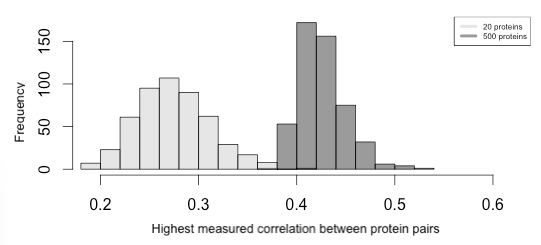
\includegraphics[width=1\textwidth]{figs/spurious_corr.png}}
\caption{Simulated experiments quantifying 20 (or 500) unrelated proteins in 100 biological samples. The histograms display the highest Pearson correlation across any pair of proteins, calculated over 500 repetitions of the simulation. Increasing the number of proteins results in higher values of Pearson correlation without any biological justification.}
\label{spur_corr}
\end{figure}

Similarly, the increased incidence of spurious correlations impedes the performance of statistical methods in Step 2, which elucidate conditional independences in the data.  The spurious correlations result in more false positives when detecting putative causal conditional dependence relationships. To illustrate, we repeated the previous simulation, again starting with 20 proteins and 100 biological samples, but this time expanding to only 100 proteins.  Instead of finding the highest  spurious correlation between pairs of proteins, we apply the a causal inference-related algorithm described in Margaritis 2003 \cite{margaritis2003learning} (which performs a series of conditional independence tests between the sets of proteins), and count the number of detected conditional dependence relationships.  As before, since we randomly draw protein concentration measurement values from a Gaussian distribution, the values are completely independent, and any conditional dependence relationship reported by this algorithm has no biological justification.  We again repeat these experiments 500 times. Figure \ref{spur_dep} shows the histograms of the counts of false positive detections of conditional dependence.  The results demonstrate that an increase in the number of proteins leads to an increase in false positive detection of putative causal conditional dependence relationships. This means that the computational methods for causal inference will fail for a typical large-scale experiment, because they cannot reliably distinguish the conditional dependence relationships from noise.

\begin{figure}[!tpb]
\centerline{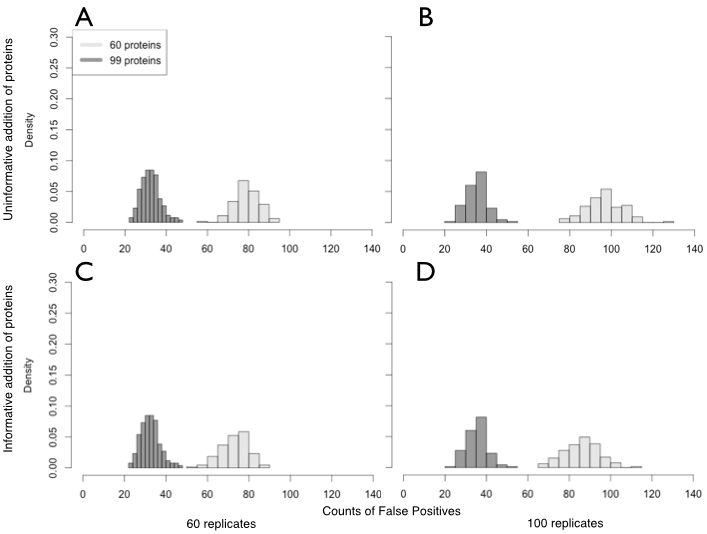
\includegraphics[width=1\textwidth]{figs/spurious_dep.png}}
\caption{As in Figure \ref{spur_corr}, but reporting the counts of false positive detections of conditional dependence.}
\label{spur_dep}
\end{figure}

An additional problem with high-throughput experiments in Step 2 is a relatively small number of biological replicates as compared to the number of analytes. While Step 1 (evaluating the set of pairwise associations) can be carried out with even a small amount of replicates, Step 2 requires that the number of replicates equals or exceeds the number of analytes.  Note the experiments demonstrated in Figure 3 had 100 replicates to its 100 proteins.  While sparse approaches working around this problem are available, quality of their results decreases drastically as the numbers of replicates fall.    

Finally, Step 3 of the workflow requires interventions to infer causal relationships from evidence of conditional dependence.  Quantifying a large number of analytes introduces a  challenge for this step as well. As the number of features grows, the number of interventions needed to fully infer causality grows, and eventually performing a sufficient perturbation experiments becomes infeasible.   We showed with the Raf-Mek-Erk example that one intervention was sufficient to infer two causal relationships. Indeed, a set of interventions on $< k$ variables may be sufficient to infer causal events between $k$ analytes. Unfortunately, both the number of biological replicates and the number of interventions im high-throughput profiling experiments is typically small.  Also, if the step 2 results in too many false positives for conditional dependence, this will adversely affect the results of step 3 regardless of the size of the dataset.


\section{III. Approaches for inferring causality from high-throughput experiments}

The problems outlined in section II paint a grim picture for causal inference in large datasets. Fortunately, these can be overcome, and effective causal inference can be a reality for large scale datasets.  We provide suggestions for the best practices below.


\begin{enumerate}
\item \textit{Limit the number of analytes.} Even though a list of analytes quantifiable with high-throughput technologies grows larger, only use a subset of measurements that are both biologically relevant and technologically accurate. The length of the list is not as important as the quality of measurements on the key parts of the system.  If the broader biological system is well understood, it may be possible to design a targeted experiment that focuses on a specific network or pathway, and ask more specific questions of the data, such as the presence of a particular regulatory event.  The more specific the question, the less data are needed to make solid causal conclusions.  

\item \textit{Profile more biological replicates.}  The high-throughput measurements should provide more samples from distinct biological sources, which come from a same underlying population, in order to achieve a sufficient statistical power, and distinguish true and spurious associations.  This fact gives advantage to technologies, such as targeted proteomics tools, that quantify fewer analytes but have a higher sample throughput.  Single cell mass cytometry is a technology deserving of special mention, where many thousands of cells per sample provide ample statistical power, though cell samples still need to be drawn from multiple individuals in order to make inferences about the population. See Sachs et al 2005 for an in depth case study of network inference with a single cell dataset. \cite{sachs2005causal}.  

\item \textit{Use prior knowledge.} Prior knowledge improves the search for conditional independence and helps to determine causality. The prior knowledge can be in form of known canonical networks, extracted, e.g. from pathway databases such as KEGG. One example of such prior information is the MAPK pathway. The prior information reduces the search space of unknown associations that need to be considered, enables a more effective use of the data, and increases the confidence in newly discovered statistical associations.  Another example of prior knowledge is contextual information, such as spatial or temporal annotations of the quantitative measurements in the cell. The contextual information can be extracted from the literature or from other complementary (and potentially noisy) datasets. The causal inference algorithms can be extended to weigh evidence of conditional dependence, depending on whether the analytes share the same spatial or temporal context. 

\item \textit{Select targeted interventions wisely.} Targeted interventions perturb individual components of the biological system.  An example is a small molecule inhibitor, which blocks the causal influence of a specific protein on its downstream components. Although effective, such targeted interventions are limited in number. Therefore, a strategic experimental design would use prior information, prioritize the interventions and the targets, and apply them to parts of the biological system that have most potential for new discovery of regulatory events.  For example, a graph with undirected edges can be inspected, to reveal which nodes have potential to reveal the most causality if perturbed. Such targeted perturbations can be applied iteratively, after an initial statistical analysis revealed areas of the network where causal inference would benefit from extra measurements and data. 


\item \textit{Consider broad-scale interventions}. Broad-scale interventions sacrifice specificity of the target to simultaneously perturb many variables in a biological system. One example of broad-scale interventions is varying experimental conditions, in order to activate multiple pathways.  Signals from endocrine, paracrine, and autocrine ligands elicit various signaling responses in hepatocytes, thus interventions that cover this range of signals gives the best picture of the broader causal network of hepatocyte signaling \cite{alexopoulos2010networks}. Similarly, interventions that go beyond receptor-level and perturb multiple components of the system bring cascading causal direct orientation deeper into the network.  Although they do not provide specific information about the downstream effects of stimulation,  broad-scale interventions can provide more causal insight. Therefore, the advantage of this approach is that it may enable elucidation of  causality across the entire system.

\end{enumerate}

This list suggests impactful approaches that can drastically improve causal inference from high-thoughput experiments, by constraining the inference task, and thus allowing for accurate
statistical inferences. For instance, the task of assessing which of all
the possible KEGG pathways is present in a dataset will be far less
error-prone than the task of assessing which of all possible
combinations of my measured variables might form a biological pathway.

How should the tools listed be used? They are most powerful when used in
combination, and in fact the lines between them are somewhat arbitrary
and frequently blurred. For instance, using item \#1 and item \#2 in
concert can be thought of as reducing the breadth and increasing the
depth of the investigation. Items \#4 and \#5 call for use of
interventions, but this task itself is complicated by measuring many
analytes. Item
\#3, prior biological knowledge, can be used to prioritize what to
target with that limited set of interventions.  Causal inference becomes possible when using these tools in combination with a sound experimental design.

\begin{acknowledgement}
We acknowledge the participants of Dagstuhl seminar 15351 "Computational Mass Spectrometry" (December 2015) (http://www.dagstuhl.de/de/programm/kalender/semhp/?semnr=15351) for their contributions to the discussion on computational manuscripts.
\end{acknowledgement}
\bibliography{write_up}
\end{document}
